\documentclass[10pt,a4paper]{article}

% --- Layout: A4 quer + 2 Seiten auf 1 Blatt ---
% --- Layout: 2 Seiten auf 1 Blatt (A4 quer) ---
\usepackage[a4paper,landscape,left=10mm,right=10mm,top=10mm,bottom=10mm]{geometry}


\usepackage{pgfpages}
\usepackage{multicol}
\usepackage{float}      % für [H]
\usepackage{caption}    % für \captionof
\usepackage{qrcode}
\usepackage{hyperref}


% --- Sprache / Text ---
\usepackage[T1]{fontenc}
\usepackage[utf8]{inputenc}
\usepackage[ngerman]{babel}

% --- Mathe / Listen ---
\usepackage{amsmath,amssymb}
\usepackage{enumitem}
\setlist[itemize]{noitemsep,topsep=0pt, partopsep=0pt}
% --- Code Styling ---
\usepackage{xcolor}
\usepackage{listings}

% Farben
\definecolor{codebg}{RGB}{248,248,248}
\definecolor{codeframe}{RGB}{220,220,220}
\definecolor{codekw}{RGB}{0,92,185}
\definecolor{codestr}{RGB}{180,60,20}
\definecolor{codecom}{RGB}{90,110,90}
\definecolor{codeid}{RGB}{70,70,70}
\definecolor{codeemph}{RGB}{155,0,90}

% Inline-Highlight (für wichtige Wörter im Text)
% --- Exam marker macros ---
\usepackage{xcolor}

\definecolor{examBlue}{RGB}{0,92,185}
\definecolor{examMagenta}{RGB}{155,0,90}

\newcommand{\pcentral}[1]{\textbf{\textcolor{examMagenta}{Zentrale Regel:}}~#1}
\newcommand{\prule}[1]{\textbf{\textcolor{examBlue}{Prüfungsregel:}}~#1}
\newcommand{\pmerke}[1]{\textbf{\textcolor{examBlue}{Prüfungsmerksatz:}}~#1}
\newcommand{\hilite}[1]{\colorbox{yellow!25}{#1}}
\newcommand{\imp}[1]{\textbf{\textcolor{codeemph}{#1}}}
\newcommand{\kw}[1]{\textbf{\textcolor{codekw}{#1}}}

% Listings: Grundstil
\lstdefinestyle{vhdl}{
  backgroundcolor=\color{codebg},
  frame=single,
  rulecolor=\color{codeframe},
  frameround=tttt,
  basicstyle=\ttfamily\fontsize{7}{8}\selectfont,
  keywordstyle=\bfseries\color{codekw},
  commentstyle=\itshape\color{codecom},
  stringstyle=\color{codestr},
  identifierstyle=\color{codeid},
  numbers=left,
  numberstyle=\tiny\color{codeid},
  numbersep=5pt,
  tabsize=2,
  showstringspaces=false,
  breaklines=true,
  breakatwhitespace=true,
  columns=fullflexible,
  keepspaces=true
}


% VHDL Sprache definieren (listings hat VHDL meist, aber so bist du safe)
\lstdefinelanguage{VHDL}{
  morekeywords={
    library,use,all,entity,is,port,generic,begin,end,architecture,of,signal,
    constant,type,record,array,process,if,then,elsif,else,when,case,others,
    loop,for,to,downto,generate,return,function,procedure,variable,shared,
    rising_edge,assert,report,severity
  },
  sensitive=true,
  morecomment=[l]--,
  morestring=[b]"
}

% Default für deine Codeblöcke
\lstset{style=vhdl,language=VHDL}

% Optional: XDC/Tcl als zweite Sprache (für Constraints)
\lstdefinestyle{xdc}{
  backgroundcolor=\color{codebg},
  frame=single,
  rulecolor=\color{codeframe},
  frameround=tttt,
  basicstyle=\ttfamily\footnotesize,
  keywordstyle=\bfseries\color{codekw},
  commentstyle=\itshape\color{codecom},
  stringstyle=\color{codestr},
  numbers=left,
  numberstyle=\tiny\color{codeid},
  numbersep=6pt,
  tabsize=2,
  showstringspaces=false,
  breaklines=true
}

% --- Grafiken ---
\usepackage{graphicx}
\usepackage{subcaption}

% --- Typografie kompakt ---
\usepackage{microtype}
\usepackage{parskip}
\setlength{\parskip}{1pt}
\setlength{\parindent}{0pt}
\renewcommand{\baselinestretch}{0.95}
\small
\setlength{\abovedisplayskip}{2pt}
\setlength{\belowdisplayskip}{2pt}
\setlength{\abovedisplayshortskip}{1pt}
\setlength{\belowdisplayshortskip}{1pt}
\linespread{0.96}


\title{Digital Microelectronics}
\author{Näf Gian Marco}
\date{\today}
\usepackage{hyperref}
\begin{document}





\begin{multicols}{3}

\maketitle
\begin{center}
\vspace{1em}


\href{https://github.com/Giamo08/Zusammenfassungen}{\texttt{github.com/Giamo08/Zusammenfassungen}}
\end{center}
% ============================================================
\section{SoC-Grundlagen und Design Flow}


\textbf{Flow:}  
System Planning \& HDL Design
$\rightarrow$ RTL Synthesis
$\rightarrow$ Netlist Linking \& Constraints
$\rightarrow$ Packing / Placement / Optimization
$\rightarrow$ Routing
$\rightarrow$ Post-Route Optimization
$\rightarrow$ Static Timing Analysis
$\rightarrow$ Bitstream Generation

\prule{%
Timing-Constraints wirken bereits ab der \hilite{Synthese} und werden in allen Folgeschritten berücksichtigt.
}


Die Zynq-7000 Plattform integriert Prozessor und FPGA auf einem Chip:
\begin{itemize}
  \item \textbf{Processing System (PS):} ARM Cortex-A9, Speichercontroller, feste Peripherie
  \item \textbf{Programmable Logic (PL):} FPGA-Logik für applikationsspezifische Beschleuniger
\end{itemize}

PS und PL sind über \hilite{AXI-Interfaces} gekoppelt und erlauben Hardware/Software-Co-Design.


Die PL stellt folgende Kernressourcen bereit:
\begin{itemize}
  \item \textbf{Logik:} CLBs mit LUTs und Flip-Flops
  \item \textbf{Speicher:} Block RAM (synchron)
  \item \textbf{Arithmetik:} DSP-Slices (MAC, Multiplizierer)
\end{itemize}
Diese Ressourcen ermöglichen hochparallele,
\hilite{datenpfadorientierte} Implementierungen.


% ============================================================
\section{SoC Constraints}

\subsection{Rolle von Constraints im SoC-Design}
HDL beschreibt primär Funktionalität, nicht physikalische oder zeitliche Eigenschaften der Hardware.  
Moderne SoC-Designs sind ohne explizite Constraints nicht korrekt implementierbar.

\imp{Merksatz (Prüfung):}  
\hilite{Constraints} liefern dem Tool alle Informationen zu \textbf{Pins, \hilite{Spannungen} und \hilite{Zeiten}}, die im HDL fehlen.

Constraints steuern Synthese, Platzierung, Routing und Timing-Optimierung.

\subsection{Arten von Constraints}
Constraints lassen sich in drei Hauptkategorien einteilen:
\begin{itemize}
  \item \textbf{Physikalische Constraints:} Pin-Zuordnung, I/O-Standards, Nutzung spezifischer FPGA-Ressourcen, Platzierung von Zellen
  \item \textbf{Timing Constraints:} Clock-Definition, Input- und Output-Delays, Timing-Ausnahmen
  \item \textbf{Konfigurations-Constraints:} Bitstream-Optionen, Konfigurationsmodi
\end{itemize}

\imp{Prüfungsregel:}  
\hilite{Timing}-\hilite{Constraints} \hilite{wirken} bereits in der Synthese, physikalische Constraints primär in der Implementierung.

\subsection{XDC-Format und Constraint-Organisation}
Vivado verwendet XDC-Dateien auf Basis von Synopsys Design Constraints (SDC).  
Constraints folgen Tcl-Syntax und werden \textbf{sequentiell} interpretiert.

Empfohlene Struktur:
\begin{itemize}
  \item Timing Assertions (Clocks, I/O-Delays)
  \item Timing Exceptions (False Paths, Multicycle Paths)
  \item Physikalische Constraints (Pins, I/O-Standards)
\end{itemize}

\textbf{Merksatz:}  
\hilite{Timing zuerst, Pins zuletzt.}

\subsection{Physikalische Constraints}
Physikalische Constraints definieren die Abbildung logischer Ports auf physische Pins sowie elektrische Eigenschaften:
\begin{itemize}
  \item Pin-Zuweisung (\texttt{PACKAGE\_PIN})
  \item I/O-Standard (\texttt{IOSTANDARD})
  \item Pull-Ups, Pull-Downs
\end{itemize}

\subsubsection*{\textcolor{codeemph}{Vorgehensschema (Prüfung)}}
\begin{enumerate}
  \item Signalrichtung bestimmen
  \item Spannung bestimmen $\rightarrow$ \texttt{IOSTANDARD}
  \item Pin zuordnen $\rightarrow$ \texttt{PACKAGE\_PIN}
  \item Reset? $\rightarrow$ \texttt{PULLUP true}
\end{enumerate}

\subsubsection*{XDC-Code-Schablone}
\begin{lstlisting}[style=xdc,emph={set_property,get_ports,PACKAGE_PIN,IOSTANDARD,PULLUP},emphstyle=\bfseries\color{codeemph}]
set_property IOSTANDARD LVCMOS33 [get_ports rst]
set_property PULLUP true [get_ports rst]
set_property PACKAGE_PIN V13 [get_ports rst]
## Timing exceptions (Exam)
set_false_path -from [get_ports rst]
# Multi-cycle (example: 2 cycles for setup, 1 for hold)
set_multicycle_path 2 -setup -from [get_cells regA] -to [get_cells regB]
set_multicycle_path 1 -hold  -from [get_cells regA] -to [get_cells regB]
\end{lstlisting}

In Sonderfällen können explizite Platzierungsconstraints (\texttt{LOC}, \texttt{BEL}) verwendet werden.

\subsection{Timing-Grundlagen und Static Timing Analysis (STA)}

Timing-Verifikation erfolgt mit \hilite{Static Timing Analysis (STA)} ohne Simulation.

\textbf{Zentrale Begriffe:}
\begin{itemize}
  \item \textbf{Clock Latency:} Verzögerung von Clock-Quelle zu Register
  \item \textbf{Clock Skew:} Laufzeitunterschied zwischen Clock-Pfaden
  \item \textbf{Clock Jitter:} Zeitliche Schwankung der Clock-Flanke
  \item \textbf{Slack:} Zeitreserve eines Pfades
\end{itemize}

\textbf{Timing-Bedingungen:}
\begin{itemize}
  \item \textbf{Setup:} Daten müssen vor aktiver Clock-Flanke stabil sein
  \item \textbf{Hold:} Daten müssen nach Clock-Flanke stabil bleiben
  \item \textbf{Pulse Width:} Mindestbreite der Clock
\end{itemize}

\prule{%
Timing ist korrekt, wenn \hilite{Setup- und Hold-Bedingungen erfüllt} sind und der \hilite{Slack $\ge 0$} ist.
}

\textbf{STA analysiert:}
\begin{itemize}
  \item Clock-to-Clock-Pfade
  \item Minimale und maximale Pfade
  \item Alle gültigen Registerpfade
\end{itemize}

\textbf{Wichtige Kennzahlen:}
\begin{itemize}
  \item \textbf{WNS (Worst Negative Slack)}
  \item \textbf{TNS (Total Negative Slack)}
\end{itemize}

\pmerke{%
STA betrachtet \hilite{alle relevanten Pfade} unabhängig von Stimuli.
}

\textbf{Setup- und Hold-Bedingungen (Prüfung):}

\[
\text{Setup: } T_{clk} \ge T_{cq}^{max} + T_{comb}^{max} + T_{setup} - T_{skew}
\]

\[
\text{Hold: } T_{cq}^{min} + T_{comb}^{min} \ge T_{hold} + T_{skew}
\]

\textbf{Slack (beide Fälle):}
\[
\text{Slack} = \text{Required Time} - \text{Arrival Time}
\]

Merksatz: Setup prüft \texttt{max}-Pfade, Hold prüft \texttt{min}-Pfade.

\begin{figure}[H]
  \centering
  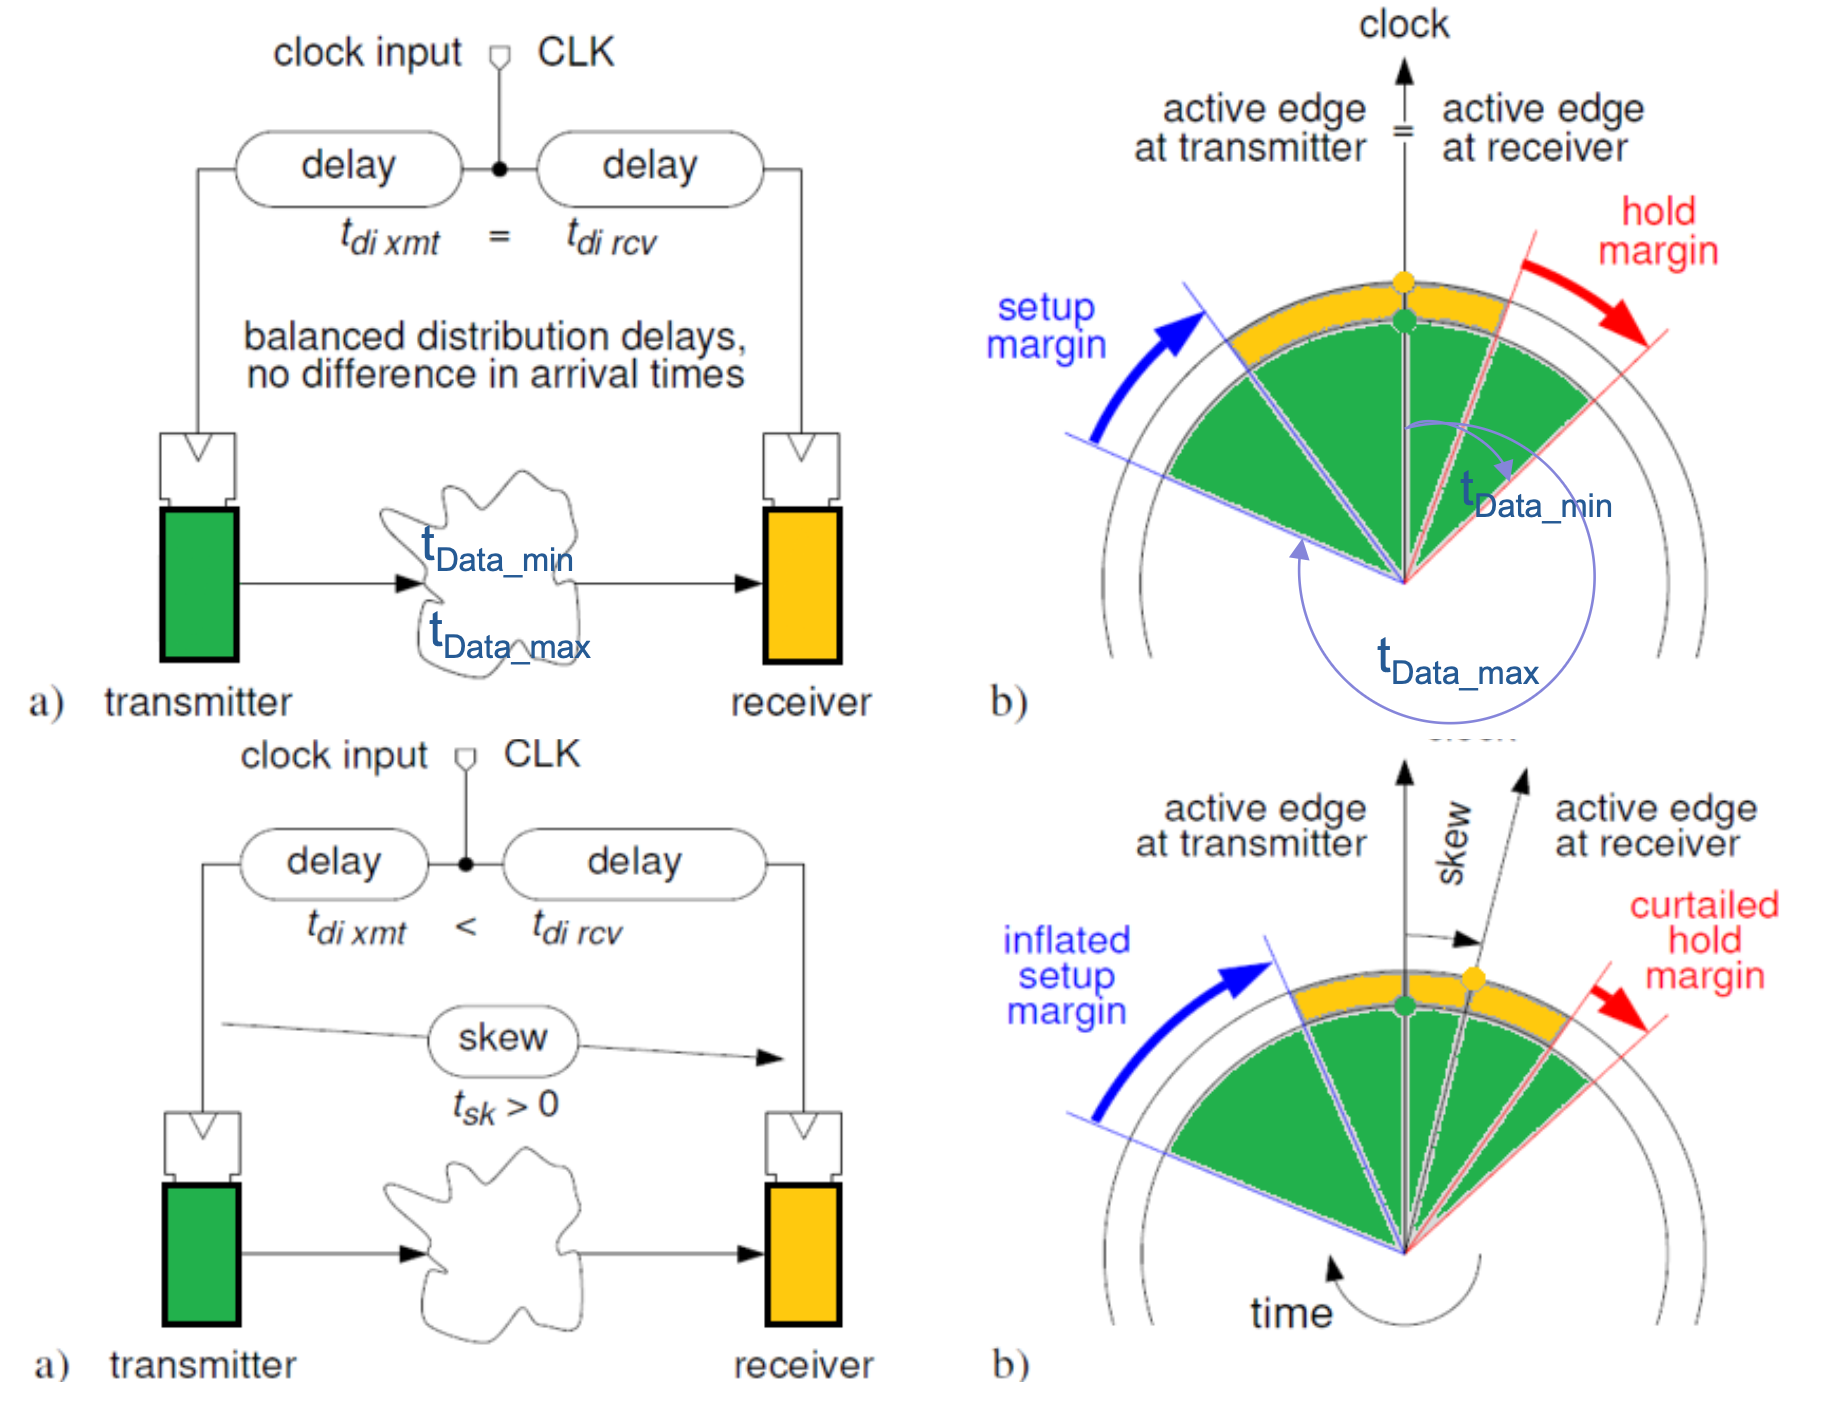
\includegraphics[width=\linewidth]{fig/L2_clock_skew.png}
  \caption{Timing-Nichtidealitäten: Latency, Skew und Jitter.}
\end{figure}

\textbf{CDC – 2-FF Synchronizer (Exam)}
\begin{lstlisting}
process(clk_b)
begin
  if rising_edge(clk_b) then
    sync1 <= sig_a;
    sync2 <= sync1;
  end if;
end process;
\end{lstlisting}
\textbf{Pipeline-Register (Timing-Fix)}
\begin{lstlisting}
process(clk)
begin
  if rising_edge(clk) then
    stage1 <= din;
    stage2 <= stage1;
  end if;
end process;
\end{lstlisting}

\subsection{Clock-Definition}
Jede relevante Clock muss explizit definiert werden.

\subsubsection*{Formel}
\[
T_{clk} = \frac{1}{f}
\]

\subsubsection*{Code-Schablone}
\begin{lstlisting}[emph={entity,architecture,process,rising_edge,signal,constant,generic,port},emphstyle=\bfseries\color{codeemph}][emph={entity,architecture,process,rising_edge,signal,constant,generic,port},emphstyle=\bfseries\color{codeemph}]
create_clock -name clk -period 10 [get_ports clk]
\end{lstlisting}

\textbf{Duty-Cycle / Waveform (Prüfung):}\\
Nicht-50\% Duty-Cycle explizit angeben:
\begin{lstlisting}
create_clock -period 5 -waveform {0 2} [get_ports clk]
\end{lstlisting}
Merksatz: Ohne \texttt{-waveform} wird 50\% angenommen.

\subsection{Input-Delay-Constraints}
Externe Signalankunftszeiten müssen spezifiziert werden.

\subsubsection*{\textcolor{codeemph}{Prüfungsformel}}
\[
t_{input\_delay} = t_{data} - t_{clk}
\]
\textbf{Prüfungs-Schema (min/max):}
\begin{itemize}
  \item \texttt{-max}: Setup-Bedingung
  \item \texttt{-min}: Hold-Bedingung
\end{itemize}
Slack (Prüfung): \\
\texttt{slack = required time - arrival time}

\subsubsection*{Code-Schablone}
\begin{lstlisting}[emph={entity,architecture,process,rising_edge,signal,constant,generic,port},emphstyle=\bfseries\color{codeemph}]
set_input_delay -clock clk 3 [get_ports data_in]
\end{lstlisting}

\subsection{Output-Delay-Constraints}
Output-Delays definieren erforderliche externe Setup- und Hold-Zeiten.

\subsubsection*{Code-Schablone}
\begin{lstlisting}[emph={entity,architecture,process,rising_edge,signal,constant,generic,port},emphstyle=\bfseries\color{codeemph}][emph={entity,architecture,process,rising_edge,signal,constant,generic,port},emphstyle=\bfseries\color{codeemph}]
set_output_delay -clock clk 5 [get_ports data_out]
\end{lstlisting}

\subsection{Wirkung von Constraints}
Constraints beeinflussen Platzierung, Routing und Optimierung direkt.

\imp{Abschluss-Merksatz (Prüfung):}  
Ohne korrekte \hilite{Constraints} kein valides Timing und kein reproduzierbares Design.

% ============================================================
\section{\hilite{System Level VHDL} und IP-\hilite{Wiederverwendung}}

\subsection{Zielsetzung von System Level VHDL}
Moderne SoC-Entwicklung erfordert skalierbare, parametrisierbare und wiederverwendbare Hardwarebeschreibungen. System Level VHDL adressiert Komplexität, Heterogenität und Time-to-Market durch Hierarchie, Modularisierung und Abstraktion.

\imp{Merksatz (Prüfung):}  
\hilite{System Level VHDL} zielt auf \textbf{\hilite{Wiederverwendung} und \hilite{Skalierung}}, nicht auf Gate-Optimierung.

Ziel ist die Wiederverwendung bewährter IP-Blöcke statt monolithischer, hardcodierter Designs.

\subsection{Grundprinzipien der Wiederverwendung}
Wiederverwendbarer VHDL-Code folgt klaren Regeln:
\begin{itemize}
  \item Keine fest kodierten Parameter
  \item Klare Schnittstellen
  \item Parametrisierung über Generics
  \item Zentrale Definition von Konstanten und Typen
  \item Saubere Dokumentation und Kommentare
\end{itemize}

\imp{Prüfungsregel:}  
\hilite{Projektweit} konstant $\Rightarrow$ \hilite{Package}. Variabel pro Instanz $\Rightarrow$ \hilite{Generic}.

Code wird typischerweise von anderen Entwicklern genutzt als vom ursprünglichen Autor. Lesbarkeit ist ein funktionales Kriterium.

\subsection{Alias, Konstanten und Generics}
Aliases verbessern die Lesbarkeit, insbesondere bei Vektorslices.

\subsubsection*{Alias – Code-Schablone}
\begin{lstlisting}[emph={entity,architecture,process,rising_edge,signal,constant,generic,port},emphstyle=\bfseries\color{codeemph}]
alias opcode : std_logic_vector(3 downto 0) is instr(15 downto 12);
\end{lstlisting}

Konstanten definieren unveränderliche Entwurfsparameter und erhöhen Konsistenz.

\subsubsection*{Konstante – Code-Schablone}
\begin{lstlisting}[emph={entity,architecture,process,rising_edge,signal,constant,generic,port},emphstyle=\bfseries\color{codeemph}][emph={entity,architecture,process,rising_edge,signal,constant,generic,port},emphstyle=\bfseries\color{codeemph}]
constant DATA_WIDTH : integer := 16;
\end{lstlisting}

Generics ermöglichen die Übergabe statischer Parameter von außen in eine Entity.

\subsubsection*{Generic – Code-Schablone}
\begin{lstlisting}[emph={entity,architecture,process,rising_edge,signal,constant,generic,port},emphstyle=\bfseries\color{codeemph}]
entity alu is
  generic ( WIDTH : integer := 16 );
  port (
    a, b : in  std_logic_vector(WIDTH-1 downto 0);
    y    : out std_logic_vector(WIDTH-1 downto 0)
  );
end entity;
\end{lstlisting}

\textbf{Merksatz:}  
\hilite{Generics} werden bei der \hilite{Instanziierung} \hilite{festgelegt} und sind zur Laufzeit konstant.

\subsection{Generate-Konstrukte}
Generate-Anweisungen erlauben die strukturierte Erzeugung mehrfacher Instanzen. In Kombination mit Generics entstehen skalierbare Hardwarestrukturen.

Typische Einsatzfälle:
\begin{itemize}
  \item Replikation identischer Verarbeitungseinheiten
  \item Parametrisierbare Breiten und Tiefen
  \item Strukturierte Arrays von Modulen
\end{itemize}

\imp{Prüfungsregel:}  
\hilite{Generate} ist \hilite{elaborationszeitlich} \hilite{wirksam} und erzeugt \textbf{echte Hardware}.

\subsubsection*{Generate – Code-Schablone}
\begin{lstlisting}[emph={entity,architecture,process,rising_edge,signal,constant,generic,port},emphstyle=\bfseries\color{codeemph}][emph={entity,architecture,process,rising_edge,signal,constant,generic,port},emphstyle=\bfseries\color{codeemph}]
gen_loop : for i in 0 to N-1 generate
  u : entity work.reg
    port map (clk => clk, d => din(i), q => dout(i));
end generate;
\end{lstlisting}

\subsection{Funktionen in VHDL}
\begin{itemize}
  \item Nur Eingangsparameter
  \item Genau ein Rückgabewert
  \item Keine Signalzuweisungen, kein wait
\end{itemize}

Geeignet für kombinatorische Logik.

\subsection{Prozeduren in VHDL}
Mehrere Ein- und Ausgänge möglich.
Primär für Testbenches, Synthese toolabhängig.

\subsection{Arrays und Records}
Records gruppieren Elemente unterschiedlicher Typen zu logischen Strukturen. Sie eignen sich für Busse, Transaktionen und strukturierte Datensätze im Systementwurf.

\subsubsection*{Record – Code-Schablone}
\begin{lstlisting}[emph={entity,architecture,process,rising_edge,signal,constant,generic,port},emphstyle=\bfseries\color{codeemph}]
type bus_t is record
  addr : std_logic_vector(15 downto 0);
  data : std_logic_vector(31 downto 0);
  we   : std_logic;
end record;
\end{lstlisting}

\subsection{Packages}
Zentrale Container für Konstanten, Typen und Funktionen.
Fördern Wiederverwendung und Konsistenz.

\subsubsection*{Package – Minimal-Schablone}
\begin{lstlisting}[emph={entity,architecture,process,rising_edge,signal,constant,generic,port},emphstyle=\bfseries\color{codeemph}][emph={entity,architecture,process,rising_edge,signal,constant,generic,port},emphstyle=\bfseries\color{codeemph}]
package defs is
  constant WIDTH : integer := 16;
  function inc(x : integer) return integer;
end package;

package body defs is
  function inc(x : integer) return integer is
  begin
    return x + 1;
  end function;
end package body;
\end{lstlisting}

\subsubsection*{Package verwenden}
\begin{lstlisting}[emph={entity,architecture,process,rising_edge,signal,constant,generic,port},emphstyle=\bfseries\color{codeemph}]
use work.defs.all;
\end{lstlisting}

Typische Anwendung: Projekt-Settings, mathematische Hilfsfunktionen, Protokollparameter.

\subsection{System-Level-Designwirkung}
System Level VHDL verschiebt den Fokus von signalorientierter Beschreibung hin zu strukturierter Systemarchitektur. Es bildet die Grundlage für IP-basierte SoC-Designs und saubere HW/SW-Partitionierung.

\imp{Abschluss-Merksatz:}  
Gute \hilite{Wiederverwendung} entsteht durch klare Schnittstellen, Generics und \hilite{Packages}.

% ============================================================
\section{\hilite{Fixed Point} Arithmetic}

\subsection{Motivation und Problemstellung}
Reale Zahlen treten in digitalen Systemen häufig auf, können jedoch in Hardware nicht direkt verarbeitet werden.  
Fixed-Point-Arithmetik ermöglicht eine effiziente Approximation reeller Werte mit endlicher Wortlänge.

\imp{Merksatz (Prüfung):}  
Bei \hilite{Fixed Point} ist der Entwickler verantwortlich für \hilite{Skalierung}, \hilite{Wortlänge} und Überlauf.

\subsection{Fixed-Point Formate und Bitwachstum (Prüfungsformeln)}

\textbf{Qn.m-Notation:}
\begin{itemize}
  \item $n$: Anzahl Integer-Bits (inkl. Vorzeichen bei signed)
  \item $m$: Anzahl Fractional-Bits
\end{itemize}

\textbf{Auflösung:}
\[
\Delta = 2^{-m}
\]

\textbf{Wertebereich:}
\[
uQn.m = [0,\; 2^n - 2^{-m}]
\]
\[
sQn.m = [-2^{n-1},\; 2^{n-1} - 2^{-m}]
\]

\pcentral{Formatregeln (prüfungsentscheidend).}

\prule{Addition/Subtraktion:}
\[
Q(n_1.m_1) + Q(n_2.m_2)
= Q(\max(n_1,n_2)+1).\max(m_1,m_2)
\]
\textit{(+1 Bit = \hilite{Guard Bit} gegen Überlauf)}

\prule{Multiplikation:}
\[
Q(n_1.m_1) \cdot Q(n_2.m_2)
= Q(n_1+n_2).(m_1+m_2)
\]

\pmerke{%
Bei signed $\times$ signed entsteht ein \hilite{redundantes Vorzeichenbit}, das meist entfernt werden kann.
}

\subsection{Ganzzahl- und Zweierkomplement-Darstellung}
Binäre Ganzzahlen werden als unsigned oder signed (Zweierkomplement) interpretiert.

Für $n$ Bit gilt:
\begin{itemize}
  \item Unsigned: $[0, 2^n - 1]$
  \item Signed: $[-2^{n-1}, 2^{n-1}-1]$
\end{itemize}

\imp{Prüfungsregel:}  
Das \hilite{Bitmuster} ist \hilite{identisch}, nur der Typ \hilite{bestimmt} die Interpretation.

\subsection{Fixed-Point-Zahlendarstellung (Qn.m)}
Fixed-Point-Zahlen besitzen einen impliziten Dezimalpunkt.  
$n$ Bits repräsentieren den ganzzahligen Anteil, $m$ Bits den fractional Anteil.

Notation:
\begin{itemize}
  \item \textbf{uQn.m}: unsigned
  \item \textbf{sQn.m}: signed
\end{itemize}

\subsubsection*{Auflösung und Wertebereich}
\[
\Delta = 2^{-m}
\]

\begin{itemize}
  \item $uQn.m = [0, 2^n - 2^{-m}]$
  \item $sQn.m = [-2^{n-1}, 2^{n-1} - 2^{-m}]$
\end{itemize}

\subsection{Skalierung und Typkonvertierung}
Reale Zahlen werden durch Skalierung in Fixed Point überführt.

\subsubsection*{\textcolor{codeemph}{Prüfungsformeln}}
\[
\text{Fixed} = \lfloor \text{Real} \cdot 2^m \rfloor
\]
\[
\text{Real} = \text{Fixed} \cdot 2^{-m}
\]

\imp{Prüfungsregel:}  
Ohne \hilite{explizite} \hilite{Typkonvertierung} keine \hilite{Arithmetik} in VHDL.

\subsection{fixed\_pkg vs. klassische Umsetzung}
Die Bibliothek \texttt{fixed\_pkg} (VHDL-2008) bietet:
\begin{itemize}
  \item Automatisches Alignment
  \item Guard Bits
  \item Kontrollierte Rundung und Sättigung
\end{itemize}

\imp{Prüfungsfokus:}  
\hilite{Prüfungen} \hilite{verlangen} \hilite{meist} die klassische Umsetzung ohne \texttt{fixed\_pkg}.

\subsection{Addition und Subtraktion}

\subsubsection*{\textcolor{codeemph}{Formatregel (Prüfung)}}
\[
Q(n_1.m_1) + Q(n_2.m_2)
= Q(\max(n_1,n_2)+1).\max(m_1,m_2)
\]

Das zusätzliche Bit ist ein \textbf{Guard Bit}.

\subsubsection*{Vorgehen ohne fixed\_pkg}
\begin{enumerate}
  \item Fractional Bits angleichen
  \item Vorzeichenerweiterung
  \item Addition
  \item Optional: Abschneiden
\end{enumerate}



\subsubsection*{Additions-Code-Schablone}
\begin{lstlisting}[emph={entity,architecture,process,rising_edge,signal,constant,generic,port},emphstyle=\bfseries\color{codeemph}][emph={entity,architecture,process,rising_edge,signal,constant,generic,port},emphstyle=\bfseries\color{codeemph}]
A_ext <= signed(A) sll 1;
B_ext <= signed(B);
Y_ext <= A_ext + B_ext;
\end{lstlisting}

\imp{Prüfungsregel:}  
\hilite{Addition} \hilite{scheitert} meist an fehlendem \hilite{Guard Bit}.

\subsection{Multiplikation}

\subsubsection*{Formatregel}
\[
Q(n_1.m_1) \cdot Q(n_2.m_2)
= Q(n_1+n_2).(m_1+m_2)
\]

Bei signed $\times$ signed entsteht ein redundantes Vorzeichenbit:
\[
Q(n_1+n_2-1).(m_1+m_2)
\]

\subsubsection*{Multiplikations-Code-Schablone}
\begin{lstlisting}[emph={entity,architecture,process,rising_edge,signal,constant,generic,port},emphstyle=\bfseries\color{codeemph}]
P <= signed(A) * signed(B);
\end{lstlisting}

\imp{Prüfungsregel:}  
\hilite{Nach} der \hilite{Multiplikation} sind \hilite{fast} immer zu viele Bits vorhanden.
Ohne \texttt{fixed\_pkg} (Prüfung):
Skalieren → Vorzeichenerweitern → Rechnen → Trunk./Round → Slice
Merksatz: Fehlerquelle Nr.1 = fehlendes Guard Bit.

\textbf{Fixed-Point Workflow (ohne fixed\_pkg)}
\begin{lstlisting}
-- scale
A_s <= signed(A) sll m;

-- sign extend + guard bit
A_ext <= A_s(A_s'left) & A_s;

-- compute
P_ext <= A_ext * B_ext;

-- truncate / round
Y <= P_ext(H downto L);
\end{lstlisting}


\subsection{Überlauf, Rundung und Sättigung}
Mögliche Effekte:
\begin{itemize}
  \item Wrap-Around (Überlauf)
  \item Sättigung
  \item Trunkierung
  \item Rundung
\end{itemize}

\imp{Prüfungsfokus:}  
\hilite{Trunkierung} und \hilite{Rundung} \hilite{unterscheiden} können.

\subsection{FIR-Filter (Prüfungsrelevanz)}
\begin{itemize}
  \item Multiplikation erzeugt Bitwachstum
  \item Akkumulation benötigt Guard Bits
\end{itemize}


\subsection{Systematische Wortlängenplanung}
Effiziente Fixed-Point-Systeme erfordern:
\begin{itemize}
  \item Analyse der Wertebereiche
  \item Konsistente Q-Formate
  \item Kontrollierte Guard Bits
\end{itemize}

\imp{Abschluss-Merksatz:}  
\hilite{Fixed Point} ist \hilite{kontrollierter} Fehler. Gute Planung schlägt hohe \hilite{Wortlänge}.


% ============================================================
\section{Custom IP Blocks: Memory}

\subsection{Einordnung und Ziel}
Speicher sind zentrale Bausteine digitaler Systeme und dominieren häufig Fläche, Energieverbrauch und Performance.  
Auf FPGAs existieren keine dedizierten ROM-Strukturen. RAM und ROM werden aus vorhandenen Hardware-Ressourcen abgebildet.

\imp{Merksatz (Prüfung):}  
\hilite{RAM} und \hilite{ROM} \hilite{unterscheiden} sich in VHDL primär durch das Zugriffsverhalten, nicht durch die Struktur.

Ziel ist die parametrisierbare Beschreibung, Initialisierung und Wiederverwendung von Speicherstrukturen als IP-Blöcke.

\subsection{Speichertypen}
Grundsätzlich wird zwischen RAM und ROM unterschieden:
\begin{itemize}
  \item \textbf{RAM}: Lesen und Schreiben zur Laufzeit
  \item \textbf{ROM}: Nur Lesen, konstante Inhalte
\end{itemize}

Technologisch:
\begin{itemize}
  \item \textbf{SRAM}: Statisch, kein Refresh
  \item \textbf{DRAM}: Dynamisch, Refresh erforderlich
\end{itemize}

FPGA-spezifisch:
\begin{itemize}
  \item \textbf{Distributed RAM} (LUT-basiert)
  \item \textbf{Block RAM} (dedizierte Hard-Macros)
\end{itemize}

\subsection{Speicherorganisation}
Logisch wird ein Speicher beschrieben durch:
\begin{itemize}
  \item \textbf{Breite}: Bits pro Wort
  \item \textbf{Tiefe}: Anzahl Wörter
\end{itemize}

\subsubsection*{\textcolor{codeemph}{Prüfungsformeln}}
\[
\text{Tiefe} = 2^{ADDR\_WIDTH}
\]
\[
\text{Gesamtbits} = \text{Breite} \cdot \text{Tiefe}
\]

\imp{Prüfungsregel:}  
\hilite{ADDR}\_\hilite{WIDTH} \hilite{bestimmt} die Anzahl Adressen, nicht die Wortbreite.

\subsection{Speicherports und Zugriffsarten}
Unterstützte Port-Typen:
\begin{itemize}
  \item \textbf{Single Port RAM}
  \item \textbf{Simple Dual Port RAM}
  \item \textbf{True Dual Port RAM}
\end{itemize}

\subsubsection*{\textcolor{codeemph}{Unterschiede (Prüfung)}}
\begin{itemize}
  \item Single Port: Lesen oder Schreiben
  \item Simple DP: ein Schreib-, ein Leseport
  \item True DP: zwei vollwertige Ports
\end{itemize}

\subsection{Zugriffsmodi bei Schreibkollisionen}
Bei gleichzeitigem Zugriff auf dieselbe Adresse:
\begin{itemize}
  \item \textbf{Write First}
  \item \textbf{Read First}
  \item \textbf{No Change}
\end{itemize}

\imp{Prüfungsregel:}  
Das \hilite{Verhalten} ist nicht \hilite{implizit}, \hilite{sondern} muss spezifiziert werden.
\textbf{RAM Write-Collision Behaviour (Exam)}
\begin{lstlisting}
process(clk)
begin
  if rising_edge(clk) then
    if we = '1' then
      ram(addr) <= din;
    end if;

    -- WRITE_FIRST
    dout <= din when we='1' else ram(addr);

    -- READ_FIRST
    -- dout <= ram(addr);

    -- NO_CHANGE
    -- if we='0' then dout <= ram(addr); end if;
  end if;
end process;
\end{lstlisting}


\subsection{Distributed RAM}
Distributed RAM nutzt LUTs (SLICEMs):
\begin{itemize}
  \item Schreiben synchron
  \item Lesen asynchron
  \item Kleine, schnelle Speicher
\end{itemize}

\imp{Prüfungsregel:}  
A\hilite{synchron}es \hilite{Lesen} $\rightarrow$ \hilite{Distributed RAM}.

\subsection{Block RAM}
Block RAM besteht aus dedizierten Hard-Macros:
\begin{itemize}
  \item 36\,kb physisch, ca. 32\,kb nutzbar
  \item Synchrones Lesen und Schreiben
  \item Unterstützt ECC und FIFO
\end{itemize}

\imp{Prüfungsregel:}  
\hilite{Synchrones} \hilite{Lesen} $\rightarrow$ \hilite{Block RAM}.

\begin{quote}\small
\textbf{Distributed RAM:} LUT-basiert, synchrones Schreiben, asynchrones Lesen.
Geeignet für kleine, schnelle Speicher. 
\textbf{Prüfungsregel:} async read $\Rightarrow$ Distributed RAM.

\textbf{Block RAM:} Dedizierte Speicherblöcke, synchrones Lesen und Schreiben.
Geeignet für große Speicher mit deterministischem Timing.
\textbf{Prüfungsregel:} sync read $\Rightarrow$ Block RAM.
\end{quote}


\subsection{VHDL-Modellierung von RAM}

\subsubsection*{Grundregeln}
\begin{itemize}
  \item Breite und Tiefe über Generics
  \item Eindimensionales Array
  \item Ein Prozess pro Port
\end{itemize}

\subsubsection*{Single Port RAM – Code-Schablone}
\begin{lstlisting}[emph={entity,architecture,process,rising_edge,signal,constant,generic,port},emphstyle=\bfseries\color{codeemph}][emph={entity,architecture,process,rising_edge,signal,constant,generic,port},emphstyle=\bfseries\color{codeemph}]
type ram_t is array (0 to DEPTH-1) of std_logic_vector(W-1 downto 0);
signal ram : ram_t;

process(clk)
begin
  if rising_edge(clk) then
    if we='1' then
      ram(addr) <= din;
    end if;
    dout <= ram(addr);
  end if;
end process;
\end{lstlisting}

\subsubsection*{True Dual Port RAM – Hinweis}
True Dual Port RAM wird häufig besser über dedizierte Block-RAM-IP realisiert.  
Eine VHDL-Modellierung mit \texttt{shared variable} ist simulatorfreundlich, aber kritisch.

\subsection{Synthesis-Attribute}
Die Implementierung kann gezielt beeinflusst werden:

\begin{lstlisting}[emph={entity,architecture,process,rising_edge,signal,constant,generic,port},emphstyle=\bfseries\color{codeemph}][emph={entity,architecture,process,rising_edge,signal,constant,generic,port},emphstyle=\bfseries\color{codeemph}]
attribute ram_style : string;
attribute ram_style of ram : signal is "block";
\end{lstlisting}

Alternativ:
\begin{lstlisting}[emph={entity,architecture,process,rising_edge,signal,constant,generic,port},emphstyle=\bfseries\color{codeemph}][emph={entity,architecture,process,rising_edge,signal,constant,generic,port},emphstyle=\bfseries\color{codeemph}]
attribute ram_style of ram : signal is "distributed";
\end{lstlisting}

\imp{Merksatz (Prüfung):}  
\hilite{Attribute} sind \hilite{Hinweise} an das \hilite{Tool}, keine funktionalen Anweisungen.

\subsection{ROM-Implementierung}
ROM unterscheidet sich von RAM nur durch konstante Inhalte.

\subsubsection*{ROM – Code-Schablone}
\begin{lstlisting}[emph={entity,architecture,process,rising_edge,signal,constant,generic,port},emphstyle=\bfseries\color{codeemph}][emph={entity,architecture,process,rising_edge,signal,constant,generic,port},emphstyle=\bfseries\color{codeemph}]
type rom_t is array (0 to 15) of std_logic_vector(7 downto 0);
constant rom : rom_t := (
  0 => x"12",
  1 => x"34",
  others => x"00"
);
\end{lstlisting}

\subsection{Speicherinitialisierung}
Möglichkeiten:
\begin{itemize}
  \item Initialisierung bei Deklaration
  \item Datei-basierte Initialisierung (.coe, .mif)
\end{itemize}

\imp{Prüfungsregel:}  
\hilite{ROM} ohne \hilite{Initialisierung} ist \hilite{inhaltlich} wertlos.

\subsection{Memory Generator IP}
Parametrisierte Speicher-IP mit wählbarer
Breite, Tiefe und Zugriffsart wird von Xilinx bereitgestellt.


\subsection{IP-Wiederverwendung und Integration}
IP-Blöcke sind parametrisierte, wiederverwendbare Einheiten.

\begin{itemize}
  \item Hard IP
  \item Firm IP
  \item Soft IP
\end{itemize}

Integration:
\begin{itemize}
  \item IP Integrator
  \item RTL-Instantiation
\end{itemize}

\begin{quote}\small
\textbf{IP-Integrator / ARM-Workflow (Zynq):}
Das Processing System (ARM) wird im IP Integrator
konfiguriert und über AXI mit Custom-IP in der
Programmable Logic verbunden.
Nach Validierung des Block Designs erfolgt die
Hardware-Generierung und der Export (XSA/HDF)
für die Software-Toolchain.
Software (BSP, Treiber, Applikation) greift über
memory-mapped Register auf die FPGA-Logik zu.
\end{quote}

% ============================================================
\section{Serial Communication Interfaces}

\subsection{Serielle Schnittstellen -- kompakte Einordnung}

\pcentral{Serielle Kommunikation spart Pins, erhöht Logikaufwand.}

\textbf{Grundklassifikation (Prüfung):}
\begin{itemize}
  \item \textbf{Topologie:} Point-to-Point, Bus
  \item \textbf{Zeitorganisation:} synchron, asynchron
  \item \textbf{Physik:} Single-Ended, differentiell
\end{itemize}

\prule{%
Serielle Schnittstellen reduzieren Pin-Anzahl, benötigen jedoch \hilite{Serialisierung und Steuerlogik}.
}

\vspace{4pt}
\textbf{Logik zu Physik:}
\begin{itemize}
  \item VHDL beschreibt \textbf{logische Signale}
  \item Elektrisches Verhalten wird durch \hilite{I/O-Pads und Constraints} festgelegt
\end{itemize}

\prule{%
Das Pad bestimmt Spannungspegel, Drive Strength und Pull-Ups, \hilite{nicht das Protokoll}.
}

\vspace{4pt}
\textbf{Spannungs- vs. Strommodus (Kurzfassung):}
\begin{itemize}
  \item \textbf{Voltage Mode:} Spannungspegel, einfach, geringere Datenrate
  \item \textbf{Current Mode:} Stromfluss, kleiner Signalhub, hohe Datenrate
\end{itemize}

\prule{%
Hohe Datenrate $\Rightarrow$ \hilite{Current Mode} (z.B. LVDS).
}

\vspace{4pt}
\textbf{LVDS (nur prüfungsrelevant):}
\begin{itemize}
  \item Differenziell
  \item Strommodus
  \item Hohe Störfestigkeit
\end{itemize}

\pmerke{%
LVDS wird über \hilite{I/O-Constraints} konfiguriert, nicht im HDL.
}

\vspace{4pt}
\textbf{Serialisierung (Minimalmodell):}
\begin{itemize}
  \item Parallel-In / Serial-Out (PISO)
  \item Serial-In / Parallel-Out (SIPO)
  \item Implementiert mit \hilite{Shiftregistern + FSM}
\end{itemize}

\prule{%
Serielle Übertragung benötigt explizite \hilite{Sende-/Empfangssteuerung}.
}


\subsection{SPI – Serial Peripheral Interface}
SPI ist eine synchrone, serielle Punkt-zu-Punkt-Schnittstelle.

Signale:
\begin{itemize}
  \item CS, SCLK, MOSI, MISO
\end{itemize}

Eigenschaften:
\begin{itemize}
  \item Master-Slave
  \item Vollduplex
\end{itemize}

Übertragungsparameter:
\begin{itemize}
  \item Clock Polarity (CPOL)
  \item Clock Phase (CPHA)
\end{itemize}

\begin{figure}[H]
  \centering
  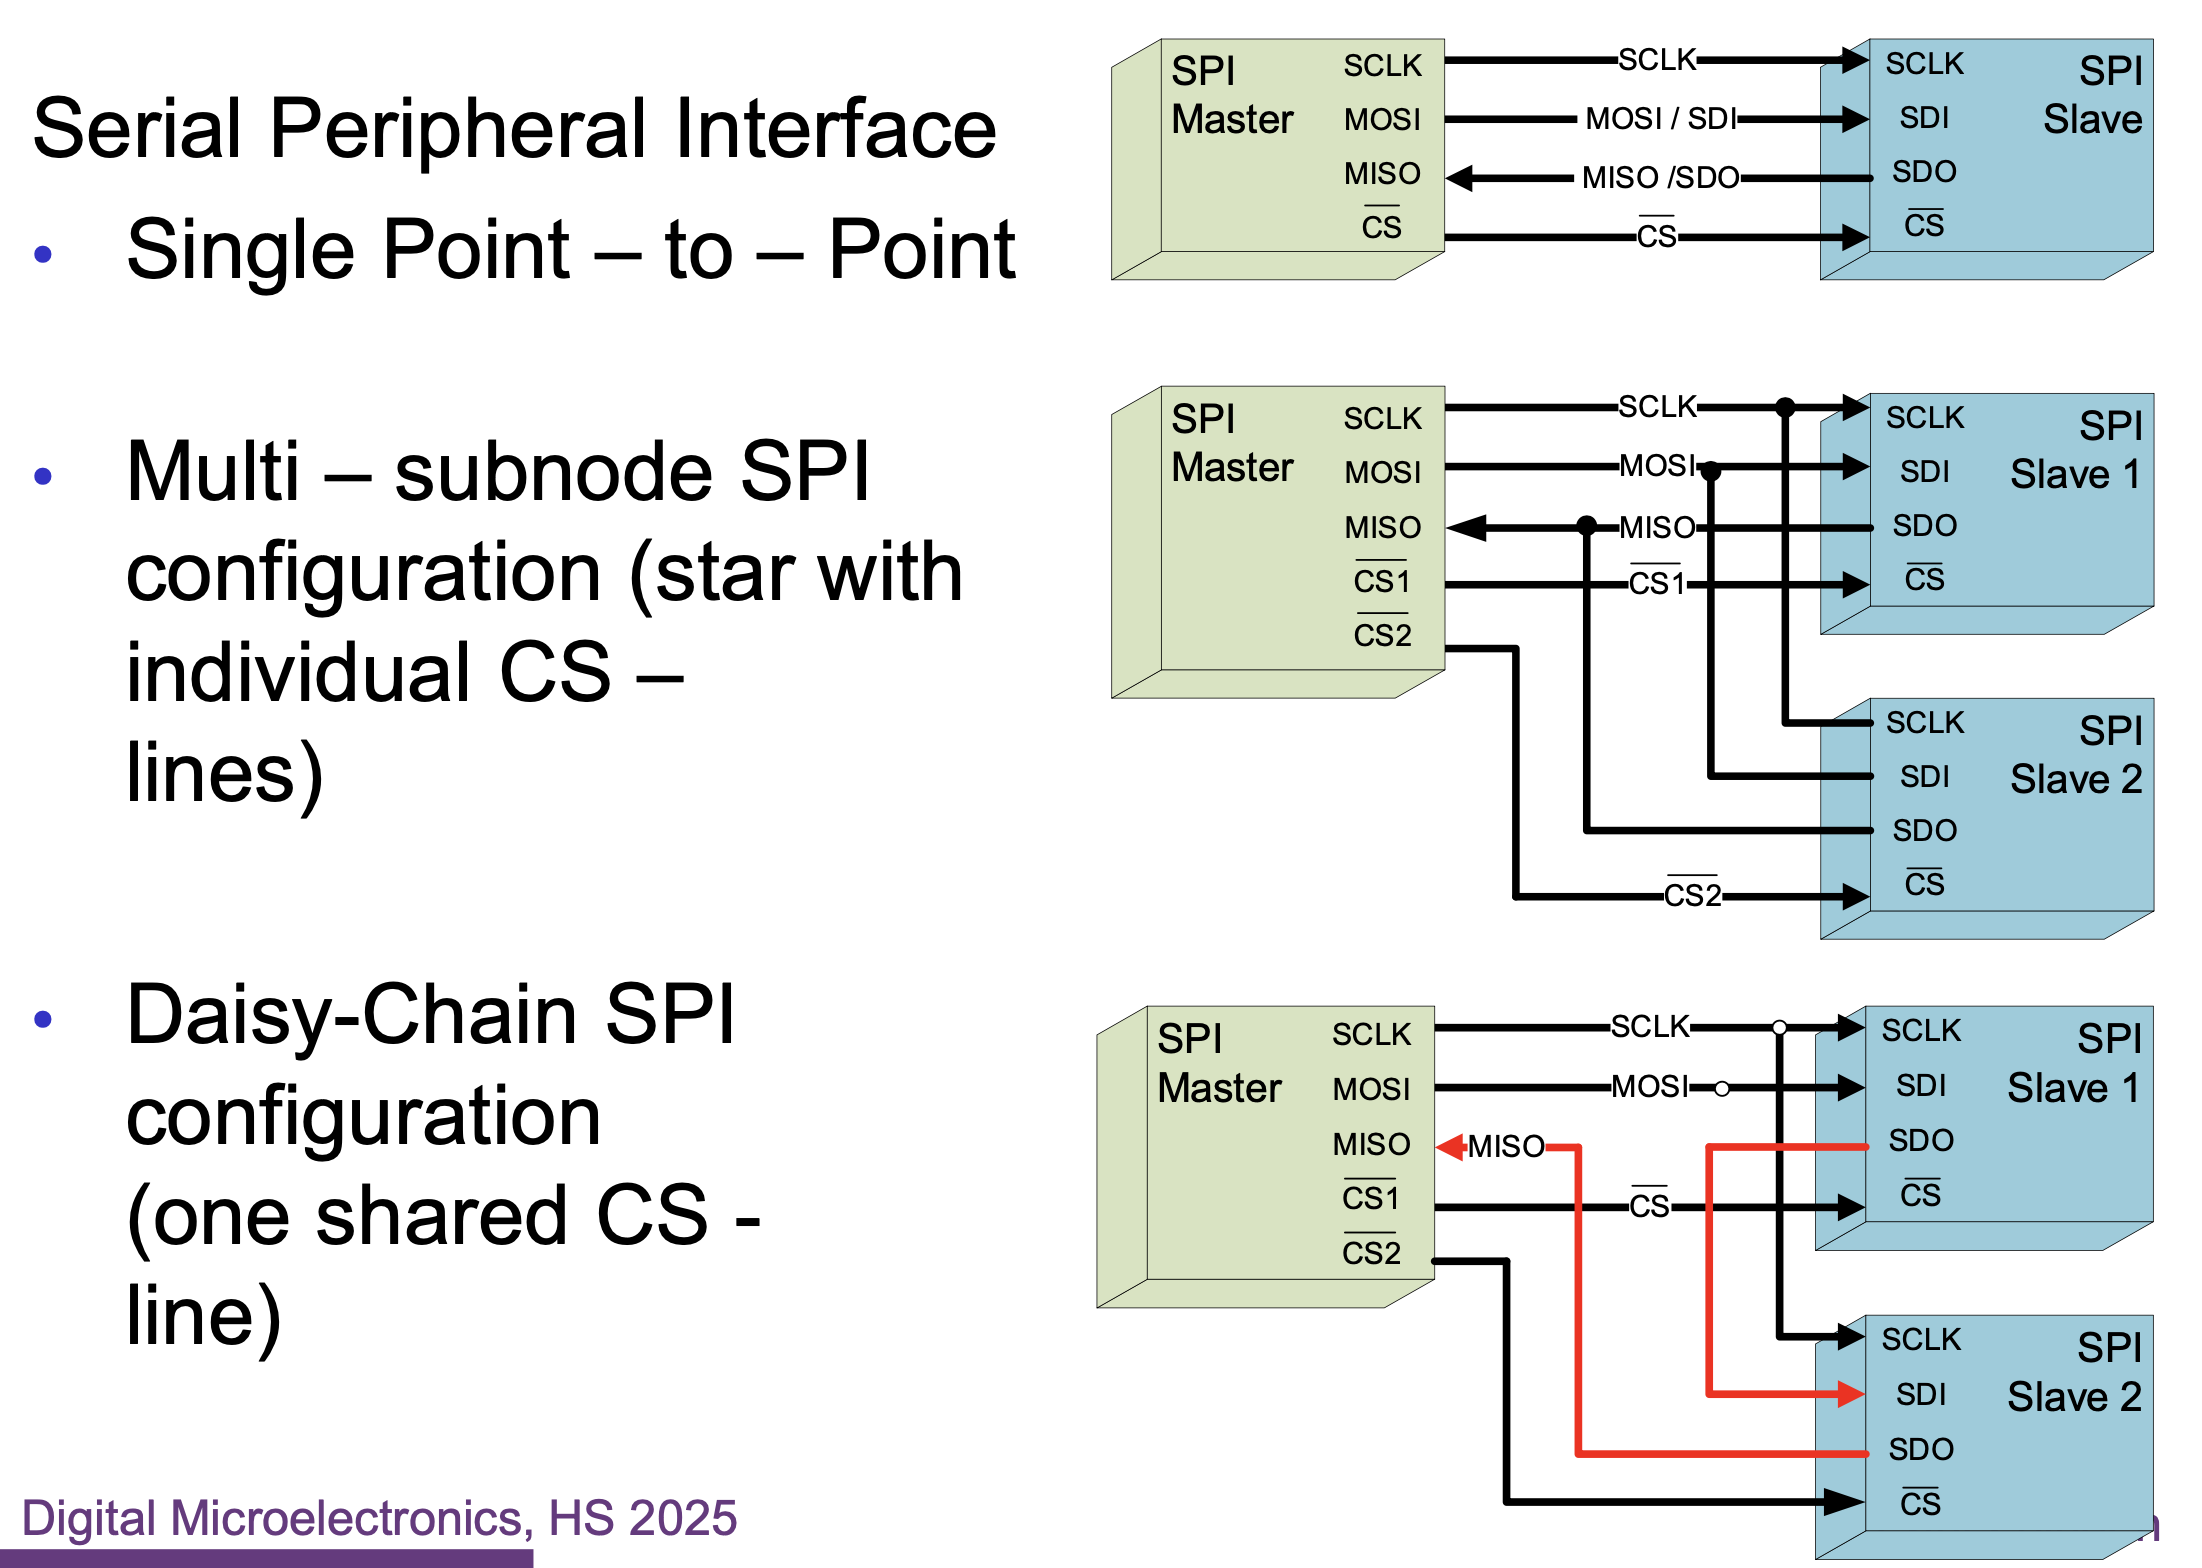
\includegraphics[width=\linewidth]{fig/L6_spi_topology.png}
  \caption{SPI-Topologien, Signale und Master-Slave-Prinzip.}
\end{figure}

\subsection{SPI-Hardwarestruktur}
SPI besteht aus Shiftregistern, Clock-Divider und FSM.
\imp{Prüfungsregel:}  
\hilite{SPI} ist \hilite{vollständig} \hilite{synchron}.

\subsection{SPI-Beschreibung in VHDL}
Die Beschreibung folgt einem festen Muster: Generics für Wortbreite und Modus, FSM zur Steuerung und Clock-Divider für SCLK.


\subsection{I\textsuperscript{2}C – Inter-Integrated Circuit}
I\textsuperscript{2}C ist eine synchrone Zweidraht-Bus-Schnittstelle.

Eigenschaften:
\begin{itemize}
  \item SDA, SCL
  \item Multi-Master, Multi-Slave
  \item Open-Drain
\end{itemize}

\subsection{I\textsuperscript{2}C (Prüfungsrelevanz)}
\begin{itemize}
  \item SDA, SCL (Open-Drain)
  \item Start/Stop bei SCL=High
  \item Arbitration über Wired-AND
\end{itemize}


Open-Drain in VHDL:
\begin{lstlisting}[emph={entity,architecture,process,rising_edge,signal,constant,generic,port},emphstyle=\bfseries\color{codeemph}][emph={entity,architecture,process,rising_edge,signal,constant,generic,port},emphstyle=\bfseries\color{codeemph}]
sda <= '0' when drive_low='1' else 'Z';
\end{lstlisting}

\subsection{UART (Einordnung)}
UART ist eine asynchrone Punkt-zu-Punkt-Schnittstelle mit Start/Stop-Bits und hat keine gemeinsame clocks.

% ============================================================
\section{Parallel On-Chip Communication}

\subsection{Einordnung paralleler Kommunikation}
Parallele Kommunikation überträgt mehrere Bits gleichzeitig über separate Leitungen.  
Sie wird primär \textbf{on-chip} eingesetzt, da physikalische Effekte off-chip die Skalierbarkeit stark begrenzen.

\imp{Merksatz (Prüfung):}  
\hilite{Parallel} = \hilite{hoher} \hilite{Durchsatz} bei kurzer Distanz.

\subsection{Serial vs. Parallel}
\imp{Prüfungsregel:}  
\hilite{Off-chip} \hilite{dominiert} \hilite{seriell}, on-chip dominiert parallel.

\subsection{Physikalische Grenzen paralleler Off-Chip-Kommunikation}
Außerhalb des Chips begrenzen physikalische Effekte den Nutzen paralleler Übertragung:

\begin{itemize}
  \item \textbf{Skew}: Laufzeitunterschiede zwischen Leitungen
  \item \textbf{Crosstalk}: Kopplung benachbarter Leitungen
  \item Hoher Pad-Bedarf
  \item Hohe Kosten
\end{itemize}

\imp{Prüfungsregel:}  
\hilite{Mehr} \hilite{Leitungen} $\rightarrow$ \hilite{mehr} Off-Chip-Probleme.

\subsection{Vorteile paralleler On-Chip-Kommunikation}
Auf dem Chip entfallen die meisten Nachteile: Keine Pads, kurze kontrollierte Leitungen, geringer Skew und keine SERDES-Strukturen.

\textbf{Merksatz:}  
\hilite{On-Chip-}\hilite{Interconnect}s sind \hilite{natürlich} parallel.

\subsection{Grundstruktur paralleler Schnittstellen}
Eine parallele Schnittstelle besteht aus:

\begin{itemize}
  \item Datenbus
  \item Steuerleitungen (Read, Write, Valid, Ready)
  \item Gemeinsamer Clock
\end{itemize}

\imp{Prüfungsregel:}  
\hilite{Parallele} \hilite{Interfaces} sind immer \hilite{synchron}.

\subsection{AXI als Standard-On-Chip-Interconnect}
AXI (Advanced eXtensible Interface) ist Teil der AMBA-Architektur von ARM und de-facto Standard für SoC-Designs.

\begin{itemize}
  \item Master-Slave
  \item Memory-Mapped
  \item Hohe Parallelität
\end{itemize}

\imp{Merksatz (Prüfung):}  
\hilite{AXI} ist \hilite{kanalbasiert}, kein \hilite{klassischer} Bus.

\subsection{AXI-Architektur}
AXI verwendet fünf unabhängige Kanäle: Write Address (AW), Write Data (W), Write Response (B), Read Address (AR) und Read Data (R).


\imp{Prüfungsregel:}  
\hilite{Read} und \hilite{Write} sind \hilite{vollständig} getrennt.

\subsection{AXI Handshake (VALID/READY)}

\pcentral{Alle AXI-Kanäle nutzen dasselbe Handshake-Schema.}

\begin{enumerate}[leftmargin=*,itemsep=0pt,topsep=2pt]
  \item \textbf{Source} setzt \hilite{VALID=1}, sobald Adresse/Daten stabil anliegen.
  \item \textbf{Destination} setzt \hilite{READY=1}, sobald sie Adresse/Daten annehmen kann.
  \item \textbf{Transfer} erfolgt an der \hilite{ersten aktiven Taktflanke}, nachdem \hilite{VALID=1} und \hilite{READY=1} gleichzeitig sind.
\end{enumerate}

\prule{%
Solange \hilite{VALID=1} und \hilite{READY=0}, müssen Adresse/Daten \textbf{stabil bleiben}.
}


\subsection{AXI-Varianten}
AXI existiert in mehreren Varianten:

\begin{itemize}
  \item \textbf{AXI4}: Vollständig, Bursts bis 256 Transfers
  \item \textbf{AXI4-Lite}: Keine Bursts, Registerzugriffe
  \item \textbf{AXI4-Stream}: Datenstrom ohne Adressen
\end{itemize}

\imp{Prüfungsregel:}  
\hilite{Register-}\hilite{IP} $\rightarrow$ \hilite{AXI4-Lite}.

\subsection{AXI-Interconnect-Topologien}

AXI-Interconnects verbinden mehrere Master und Slaves über definierte Topologien.
Je nach Richtung sind unterschiedliche Kontrollmechanismen notwendig.

\textbf{1-to-1:}
Ein Master direkt mit einem Slave verbunden(ohhne Arbitration oder Adressdekodierung).


\textbf{N-to-1 (Arbitration):}
Mehrere Master greifen auf einen Slave zu(z.B. Speichercontroller, nur ein Master darf gleichzeitig senden).


\textbf{1-to-M (Decoding/Routing):}
Ein Master greift auf mehrere Slaves zu(z.B. CPU auf verschiedene Peripheriekomponenten, Adressdekodierung, keine Arbitration).

\textbf{N-to-M:}
Mehrere Master greifen auf mehrere Slaves zu(Arbitration und Adressdekodierung).

\prule{%
AXI-Interconnects sind 
punkt-zu-punkt kanalbasiert; 
Arbitration und Routing erfolgen im Interconnect, nicht im Master.
}

\subsection{AXI auf Zynq}
PS und PL sind über General Purpose (GP), High Performance (HP) und Accelerator Coherency Port (ACP) AXI-Ports verbunden.


\subsection{AXI3 vs. AXI4}
Im Zynq:
\begin{itemize}
  \item PS nutzt AXI3
  \item Xilinx-IP nutzt AXI4
\end{itemize}

\imp{Prüfungsregel:}  
\hilite{Protokollkonverter} \hilite{lösen} \hilite{Inkompatibilitäten}.

\subsection{AXI-IP-Erstellung}
Gängige Vorgehensweisen:
\begin{itemize}
  \item Separater AXI-Interface-Block + User-Logik
  \item AXI-Peripheral-Template
\end{itemize}

\subsection{Register-basierte Kommunikation}
Kommunikation erfolgt über Memory-Mapped Register:

\begin{itemize}
  \item CPU schreibt Register
  \item Logik liest Register
  \item Logik schreibt Status
  \item CPU liest Status
\end{itemize}

\subsection{FPGA–Processor-Kommunikation}
Integration erfolgt über:
\begin{itemize}
  \item Hardware-Export
  \item BSP-Generierung
  \item Automatische Address-Header
\end{itemize}

\imp{Abschluss-Merksatz:}  
\hilite{AXI} \hilite{verbindet} \hilite{Software-Welt} und FPGA-Logik deterministisch.



% ============================================================
\section{Debugging and Verification of SoC}

\subsection{Einordnung der Verifikation}
Design Verification ist ein zentraler Bestandteil moderner SoC-Entwicklung und beansprucht häufig über 50\,\% der Entwicklungszeit.

\imp{Prüfungsmerksatz:}  
\hilite{Verifikation} \hilite{prüft} \emph{richtiges Verhalten}, nicht Performance oder \hilite{Timing}.

In dieser Vorlesung wird ausschließlich \textbf{funktionale Verifikation} betrachtet.

\subsection{Funktionale Verifikation}
Funktionales Verhalten lässt sich beschreiben als:
\[
y = f(x, \text{state})
\]

\imp{Prüfungsregel:}  
\hilite{Verifikation} \hilite{prüft}, ob für \hilite{gegebene} Eingänge und Zustände die korrekten Ausgänge entstehen.

\subsection{Exhaustive Verification}
Exhaustive Verification testet \textbf{alle möglichen Eingangskombinationen}.

\subsubsection*{\textcolor{codeemph}{Prüfungsformel}}
Für $n$ unabhängige Eingänge gilt:
\[
N = 2^n
\]
Erweitert (Prüfung): \\
\[
N = 2^{(n_{inputs} + n_{state})}
\]
Beispiel: 1 Input + 2 Zustände → $2^3 = 8$ Testvektoren


\imp{Prüfungsregel:}  
\hilite{Exhaustive} \hilite{Verification} ist \hilite{theoretisch} korrekt, praktisch unmöglich.

\subsection{Pragmatische Verifikationsstrategie}
Da Exhaustive Verification nicht realisierbar ist, wird ein Kompromiss gewählt:

\begin{itemize}
  \item Assertion-Based Verification
  \item Gezielte Testfälle
  \item Zufällige Stimuli
  \item Trennung von Design und Test
\end{itemize}

\textbf{Merksatz:}  
\hilite{Ziel} ist \hilite{hohe} \hilite{Fehlerabdeckung}, nicht Vollständigkeit.

\subsection{Assertion-Based Verification}
Assertions sind eingebaute Konsistenzprüfungen.

\subsubsection*{Typische Assertions}
\begin{itemize}
  \item Illegale FSM-Zustände
  \item Ungültige Adressen
  \item Über- und Unterläufe
\end{itemize}

\subsubsection*{Assertion – Code-Beispiel}
\begin{lstlisting}[emph={entity,architecture,process,rising_edge,signal,constant,generic,port},emphstyle=\bfseries\color{codeemph}][emph={entity,architecture,process,rising_edge,signal,constant,generic,port},emphstyle=\bfseries\color{codeemph}]
assert addr < MAX_ADDR
  report "Address out of range"
  severity error;
\end{lstlisting}

\imp{Prüfungsregel:}  
\hilite{Assertions} sind nicht für die \hilite{Synthese} \hilite{bestimmt}.

\subsection{Testfälle und Stimuli}
Effektive Testfälle decken unterschiedliche Szenarien ab:

\begin{itemize}
  \item Normalbetrieb
  \item Grenzfälle
  \item Fehlerfälle
  \item Zufällige Daten
\end{itemize}

\imp{Prüfungsregel:}  
\hilite{Grenzwerte} \hilite{finden} \hilite{mehr} Fehler als Mittelwerte.

\subsection{Golden Model}
Ein Golden Model liefert Referenzergebnisse für gegebene Stimuli.

\subsubsection*{\textcolor{codeemph}{Prüfungsregel}}
DUT erzeugt Ergebnis $\rightarrow$ Golden Model erzeugt Erwartungswert $\rightarrow$ Automatischer Vergleich.


Ohne Golden Model keine skalierbare Verifikation.

\subsection{Test-Bench-Organisation}
Strukturierte Test-Benches folgen festen Regeln:

\begin{itemize}
  \item Periodische Clock
  \item Genau ein Stimulus pro Takt
  \item Antwortauswertung synchron zur Clock
\end{itemize}

\subsubsection*{Clock – Minimal-Code}
\begin{lstlisting}[emph={entity,architecture,process,rising_edge,signal,constant,generic,port},emphstyle=\bfseries\color{codeemph}][emph={entity,architecture,process,rising_edge,signal,constant,generic,port},emphstyle=\bfseries\color{codeemph}]
clk <= not clk after 10 ns;
\end{lstlisting}

\imp{Prüfungsregel:}  
Un\hilite{synchron}\hilite{isierte} \hilite{Test-Benches} erzeugen Scheinergebnisse.
\textbf{Testbench – Exam Skeleton}
\begin{lstlisting}
signal clk : std_logic := '0';

clk <= not clk after 10 ns;

stim : process
begin
  rst <= '1'; wait for 20 ns;
  rst <= '0';
  din <= x"55"; wait for 20 ns;
  assert dout = x"55"
    report "Mismatch"
    severity error;
  wait;
end process;
\end{lstlisting}

\subsection{Automatische Auswertung}
Visuelle Inspektion ist unzureichend.

\subsubsection*{\textcolor{codeemph}{Prüfungsrezept}}
Stimulus erzeugen $\rightarrow$ DUT simulieren $\rightarrow$ Ergebnis speichern $\rightarrow$ mit Golden Model vergleichen.


\textbf{Merksatz:}  
Was nicht \hilite{automatisch} \hilite{prüft}, \hilite{skaliert} nicht.

\subsection{File-basierte Test-Benches}
Erlauben große Testmengen.
Nur in Testbenches erlaubt.


\imp{Prüfungsregel:}  
\hilite{File-I}/O ist \hilite{Testbench}-\hilite{only}.

\subsection{Simulation und Modelle}
Funktionale Simulation:
\begin{itemize}
  \item VHDL oder Verilog
\end{itemize}

Timing-Simulation:
\begin{itemize}
  \item Nur Verilog
\end{itemize}

\imp{Prüfungsregel:}  
\hilite{VHDL} \hilite{besitzt} keine simprim-\hilite{Timing}bibliothek.

\subsection{Debugging in Simulation}
Simulation erlaubt vollständige Sichtbarkeit. Mit den Werkzeugen Signal-Inspection, Breakpoints, Step-by-Step und Signal-Forcing können Fehler systematisch gefunden werden.

\subsection{Voraussetzungen zum Finden eines Fehlers}
Ein Fehler wird nur gefunden, wenn alle drei Bedingungen erfüllt sind:

\begin{enumerate}
  \item \textbf{Sensitization}: Fehler wird aktiviert
  \item \textbf{Propagation}: Fehler breitet sich aus
  \item \textbf{Observation}: Fehler ist sichtbar
\end{enumerate}

\subsubsection*{\textcolor{codeemph}{Prüfungsmerksatz}}
Kein Output-Unterschied $\Rightarrow$ kein gefundener Fehler.

\subsection{Stuck-at-Fehlermodell}
Ein Signal ist permanent auf 0 oder 1 festgesetzt.

\subsubsection*{\textcolor{codeemph}{Prüfungsrezept}}
\begin{itemize}
  \item Eingang so wählen, dass sa0/sa1 wirksam wird
  \item Pfad bis Ausgang freischalten
  \item Ausgang vergleichen
\end{itemize}

\imp{Prüfungsregel:}  
\hilite{Stuck-at} ist ein \emph{logisches}, kein \hilite{physikalisches} \hilite{Modell}.Kein Output-Unterschied $\Rightarrow$ kein gefundener Fehler.

\subsection{Debugging in Emulation}
Auf Hardware sind interne Signale nicht direkt sichtbar.

\subsubsection*{Xilinx-Werkzeuge}
\begin{itemize}
  \item \textbf{VIO}: Setzen und Lesen interner Signale
  \item \textbf{ILA}: Logikanalysator im FPGA
\end{itemize}

\imp{Prüfungsregel:}  
\hilite{ILA} \hilite{ersetzt} den \hilite{Simulator} auf Hardware.

\subsection{Hardware/Software Co-Debugging}
In SoCs ist gekoppeltes Debugging möglich.

\subsubsection*{Mechanismus}
\begin{itemize}
  \item Software-Breakpoint triggert ILA
  \item ILA-Trigger stoppt CPU
\end{itemize}

\imp{Abschluss-Merksatz:}  
\hilite{Gute} \hilite{Verifikation} \hilite{findet} Fehler früh, billig und reproduzierbar.

%===========================================================
\section{Exam Code Templates}
\subsection{XDC: Physical + Timing (Skeleton)}
\begin{lstlisting}[style=xdc,language={},emph={set_property,IOSTANDARD,PACKAGE_PIN,PULLUP,create_clock,set_input_delay,set_output_delay,get_ports,get_clocks},emphstyle=\bfseries\color{codeemph}]
## Physical constraints
set_property IOSTANDARD LVCMOS33 [get_ports {clk rst}]
set_property PACKAGE_PIN W17    [get_ports clk]
set_property PACKAGE_PIN W20    [get_ports rst]
set_property PULLUP true        [get_ports rst]

## Clock
create_clock -period 5.0 [get_ports clk]

## Input delays
set_input_delay  -clock clk -min 1.0 [get_ports x[*]]
set_input_delay  -clock clk -max 2.5 [get_ports x[*]]

## Output delays
set_output_delay -clock clk -min 0.5 [get_ports y[*]]
set_output_delay -clock clk -max 2.0 [get_ports y[*]]
\end{lstlisting}

\subsection{VHDL: Simple Dual Port RAM (Block RAM inference)}
\begin{lstlisting}[language=VHDL,emph={generic,ADDR_WIDTH,DATA_WIDTH,ram_style,process,rising_edge,shared,to_integer,unsigned},emphstyle=\bfseries\color{codeemph}]
library ieee;
use ieee.std_logic_1164.all;
use ieee.numeric_std.all;

entity sdp_ram is
  generic(
    ADDR_WIDTH : positive := 16;
    DATA_WIDTH : positive := 8
  );
  port(
    clk_wr  : in  std_ulogic;
    clk_rd  : in  std_ulogic;
    we      : in  std_ulogic;
    addr_wr : in  std_ulogic_vector(ADDR_WIDTH-1 downto 0);
    addr_rd : in  std_ulogic_vector(ADDR_WIDTH-1 downto 0);
    din     : in  std_ulogic_vector(DATA_WIDTH-1 downto 0);
    dout    : out std_ulogic_vector(DATA_WIDTH-1 downto 0)
  );
end entity;

architecture rtl of sdp_ram is
  type mem_t is array (0 to 2**ADDR_WIDTH - 1) of std_ulogic_vector(DATA_WIDTH-1 downto 0);
  shared variable mem : mem_t;

  attribute ram_style : string;
  attribute ram_style of mem : variable is "block";
begin
  -- Write port (sync)
  p_wr : process(clk_wr)
  begin
    if rising_edge(clk_wr) then
      if we = '1' then
        mem(to_integer(unsigned(addr_wr))) := din;
      end if;
    end if;
  end process;

  -- Read port (sync)
  p_rd : process(clk_rd)
  begin
    if rising_edge(clk_rd) then
      dout <= mem(to_integer(unsigned(addr_rd)));
    end if;
  end process;
end architecture;
\end{lstlisting}

\subsection{VHDL: I2C Open-Drain (one wire)}
\begin{lstlisting}[language=VHDL,emph={inout,'Z',process},emphstyle=\bfseries\color{codeemph}]
library ieee;
use ieee.std_logic_1164.all;

entity i2c_line is
  port(
    sda      : inout std_logic;
    drive_lo : in    std_logic;  -- '1' => pull low
    sda_in   : out   std_logic
  );
end entity;

architecture rtl of i2c_line is
begin
  -- Open-drain: never drive '1'
  sda    <= '0' when drive_lo = '1' else 'Z';
  sda_in <= sda;
end architecture;
\end{lstlisting}

\subsection{VHDL: AXI4-Lite Registerbank (minimal)}
\begin{lstlisting}[language=VHDL,emph={AWVALID,AWREADY,WVALID,WREADY,BVALID,BREADY,ARVALID,ARREADY,RVALID,RREADY,ADDR,WDATA,RDATA,process,rising_edge},emphstyle=\bfseries\color{codeemph}]
library ieee;
use ieee.std_logic_1164.all;
use ieee.numeric_std.all;

entity axi_lite_regs is
  generic(ADDR_W : positive := 6); -- byte address width
  port(
    aclk    : in  std_ulogic;
    aresetn : in  std_ulogic;

    -- Write address
    awvalid : in  std_ulogic;
    awready : out std_ulogic;
    awaddr  : in  std_ulogic_vector(ADDR_W-1 downto 0);

    -- Write data
    wvalid  : in  std_ulogic;
    wready  : out std_ulogic;
    wdata   : in  std_ulogic_vector(31 downto 0);

    -- Write response
    bvalid  : out std_ulogic;
    bready  : in  std_ulogic;

    -- Read address
    arvalid : in  std_ulogic;
    arready : out std_ulogic;
    araddr  : in  std_ulogic_vector(ADDR_W-1 downto 0);

    -- Read data
    rvalid  : out std_ulogic;
    rready  : in  std_ulogic;
    rdata   : out std_ulogic_vector(31 downto 0)
  );
end entity;

architecture rtl of axi_lite_regs is
  type regfile_t is array (0 to 7) of std_ulogic_vector(31 downto 0);
  signal regs : regfile_t := (others => (others => '0'));

  signal aw_hs, w_hs, ar_hs : std_ulogic;
  signal wr_addr_idx, rd_addr_idx : integer range 0 to 7;
begin
  wr_addr_idx <= to_integer(unsigned(awaddr(5 downto 2))); -- word aligned
  rd_addr_idx <= to_integer(unsigned(araddr(5 downto 2)));

  awready <= '1';
  wready  <= '1';
  arready <= '1';

  aw_hs <= awvalid and awready;
  w_hs  <= wvalid  and wready;
  ar_hs <= arvalid and arready;

  p_axi : process(aclk)
  begin
    if rising_edge(aclk) then
      if aresetn = '0' then
        regs   <= (others => (others => '0'));
        bvalid <= '0';
        rvalid <= '0';
        rdata  <= (others => '0');
      else
        -- default: clear responses when accepted
        if bvalid = '1' and bready = '1' then bvalid <= '0'; end if;
        if rvalid = '1' and rready = '1' then rvalid <= '0'; end if;

        -- write: accept address+data in same cycle (minimal model)
        if (aw_hs = '1') and (w_hs = '1') then
          regs(wr_addr_idx) <= wdata;
          bvalid <= '1';
        end if;

        -- read: respond on address handshake
        if ar_hs = '1' then
          rdata  <= regs(rd_addr_idx);
          rvalid <= '1';
        end if;
      end if;
    end if;
  end process;
end architecture;
\end{lstlisting}

\subsection{Exam Code Patterns (Fixed Point \& Package)}

\begin{lstlisting}[language=VHDL]
-- Package: zentrale Definitionen
package exam_pkg is
  constant W : integer := 8;
  function add_fp(a,b : signed(W-1 downto 0)) return signed;
end package;

package body exam_pkg is
  function add_fp(a,b : signed(W-1 downto 0)) return signed is
    variable ext : signed(W downto 0); -- Guard Bit
  begin
    ext := (a(a'left) & a) + (b(b'left) & b);
    return ext(W-1 downto 0); -- Trunkierung
  end function;
end package body;

-- Nutzung im synchronen Prozess
use work.exam_pkg.all;

process(clk)
begin
  if rising_edge(clk) then
    y <= add_fp(a,b);
  end if;
end process;
\end{lstlisting}

\textbf{Schieberegister (Shift Register)}
\begin{lstlisting}
process(clk)
begin
  if rising_edge(clk) then
    if rst='1' then
      reg <= (others => '0');
    elsif en='1' then
      reg <= reg(reg'left-1 downto 0) & din;
    end if;
  end if;
end process;
\end{lstlisting}

\textbf{Register mit Enable (Latch-sicher)}
\begin{lstlisting}
process(clk)
begin
  if rising_edge(clk) then
    q <= q; -- default
    if en='1' then
      q <= d;
    end if;
  end if;
end process;
\end{lstlisting}

\textbf{Reset-Varianten (Prüfung)}
\begin{lstlisting}
-- synchronous reset
if rising_edge(clk) then
  if rst='1' then
    q <= '0';
  else
    q <= d;
  end if;
end if;

-- asynchronous reset
if rst='1' then
  q <= '0';
elsif rising_edge(clk) then
  q <= d;
end if;
\end{lstlisting}
\textbf{Kombinatorischer Prozess (vollständig)}
\begin{lstlisting}
process(a,b,sel)
begin
  y <= a; -- default
  if sel='1' then
    y <= b;
  end if;
end process;
\end{lstlisting}
\textbf{FSM – Exam Template (Moore)}
\begin{lstlisting}
type state_t is (IDLE, RUN, DONE);
signal state, state_n : state_t;

-- state register
process(clk)
begin
  if rising_edge(clk) then
    if rst='1' then
      state <= IDLE;
    else
      state <= state_n;
    end if;
  end if;
end process;

-- next state + output logic
process(state, start)
begin
  state_n <= state;
  case state is
    when IDLE =>
      if start='1' then state_n <= RUN; end if;
    when RUN =>
      state_n <= DONE;
    when DONE =>
      state_n <= IDLE;
  end case;
end process;
\end{lstlisting}

\textbf{Clock Enable vs. Gated Clock}
Clock Enable bevorzugen. Gated Clock vermeidet man wegen Glitches.

\end{multicols}

\end{document}
